\documentclass{article}
\usepackage[utf8]{inputenc}
\usepackage{bm}
\usepackage{amsmath}
\usepackage{graphicx}

\title{The ground state search of the Co-Re-Ti system and its potential as a super alloy}
\author{Johnathon Rackham}
\date{February 2017}
\linespread{2}


\begin{document}

\maketitle

\begin{abstract}
Due to their superior strength at high temperatures, super alloys play a vital role in the aerospace industry with the application of jet turbine engines. The ternary alloy Co-Re-Ti has recently emerged as a candidate super alloy that could compete with the traditional Ni-based alloys. Here we investigate the thermodynamic stability of the Co-Re-Ti system using a combination of first-principles calculations and cluster expansion. The cluster expansion is a model that can quickly calculate the energy of crystal structures of large atomic configurations. This makes cluster expansion a convenient tool for searching through a large number of candidate configurations. Quantum Espresso was used to calculate the formation energies for 998 candidate atomic configurations. These energies were then used to train an Ising-like model called the cluster expansion. The cluster expansion method was then used to quickly calculate the formation energies of one million candidate configurations. The convex hull reveals several ground states at Co-rich concentrations. Thermodynamic monte carlo reveals transition temperatures above 2300 K, making this system a viable candidate for super alloy applications. 
\end{abstract}

\section{Introduction}
The high strength of super alloys at high temperatures makes them very desirable to the aerospace industry. For instance, the blades of a jet turbine engine are built from a super alloy and the limitations of this alloy are one of the factors that determines the efficiency of the jet turbine engine. The alloy traditionally used in this setting is nickle based and derives its strength from the ordering of its two phased structure at operating temperatures. The crystal lattices of the two phases are both face centered cubic (fcc) and the small lattice parameter mismatch allows for the phases to lock together rather than form amorphous grains as commonly found in other metals at this temperature.
	
While traditional super alloys are nickle based, recent research suggest that there is a possibility for more tightly bound compounds containing cobalt. Researchers at Duke University preformed a high through put search by taking the crystal structure found in nickle based alloys and replacing the nickle with cobalt atoms. They then continued to swap out the alloying atoms and calculating the configuration energy of the compound. Their results indicated that Cobalt-Rhenium-Titanium (Co-Re-Ti) is a promising candidate for having super alloy like structures in the cobalt rich concentration region. This work is a ground state search of the Co-Re-Ti system to determine what structures are likely to be present in the cobalt rich region and project what the high temperature behavior of those select configurations might be.


\section{Theory}
\subsection{Density Functional Theory}
The macroscopic properties of materials are a direct result of their atomic configurations. An examination of a material's atomic configuration, particularly the energy of the materials unit cell, can provide information to predict how that material behaves \cite{stokes2000solid}. The determination of an atomic configuration's energy is a complex problem that needs quantum mechanics to adequately describe. Because there are multiple atoms, all with numerous electrons, this constitutes a many body quantum mechanics problem. Density Functional Theory (DFT) allows for a transition from using wavefunctions defined by the electron positions to wavefunctions using electron density\cite{sholl2011density}.
While the specifics of DFT is beyond the scope of this paper, a brief discussion on the its basic qualities and applications is necessary. In the case of examining a bulk material, DFT is useful because it provides an accurate, first principles method of determining configuration energy. The many bodied nature of the problem makes it infeasible to calculate configuration energy using standard quantum mechancis, i.e Schroedinger's equation. In order to describe the problem using Schroedinger's equation one needs to know the electron positions, but in order to know where the electrons are likely to be we need to know the wavefunctions. This in and of itself is not an insurmountable problem. For a small number of bodies a self consistency algorithm can successfully be used to determine the wavefunctions and subsequently, configuration energy\cite{ram2004schrodinger}. However, when the shear number of electrons and atoms is taken into account it becomes hard to justify the time and resources required, even though the algorithms would in theory work. A more practical approach was proven to work by Hohenberg and Kohn through the development of two theorems\cite{PhysRev.136.B864}. The first Hohenberg-Kohn theorems (H-K) show that the ground state properties of systems containing many bodies can be uniquely determined by electron densities which are functions of only three spatial coordinates. The second H-K theorem provides an energy functional that is minimized with the correct ground state electron density.
The work of Hohengerg and Kohn provides a method of efficiently solving the many bodied quantum problem within application scope of material studies. The implementation of the H-K theorems and self-consistency algorithms is a non trivial computational pursuit and this work makes use of the established framework that the Quantum Espresso software suite provides to handle the necessary first principles calculations\cite{giannozzi2009quantum}

(Note: This section probably needs to be expanded but I am not sure how indepth I can go regarding this topic and not get completely derailed)

\subsection{Cluster Expansion}

Let us examine the case of a simple binary alloy with a two dimensional square lattice structure. Most metallic alloys maintain a consistent parent lattice structure across multiple phases [citation]. Because the lattice structure is known, we know where each atom is located in space ($\bm{r_1}, . . .,\bm{r_n}$) just not which type, or species, of atom occupies that particular point in space. The Born-Oppenheimer approximation assumes that the nuclei of the atoms are fixed and that the electrons are essentially in their ground states[citation]. This approximation allows us to then describe the energy of a configuration as just a function of which atoms occupy which lattice positions
$$E_{BO}^{gs}(\bm{r_1}, . . .,\bm{r_m})\rightarrow E_{conf}(Z_1,...,Z_{m})$$

\noindent where $Z_m$ denotes the atom species at the position of equivalent index ($\bm{r_m} \rightarrow Z_m$). For a binary system consisting of atoms of species A, and atoms of species B, the complexity of the function can be further reduced. Because there are only two differing species of atoms on the lattice $Z$ can only take one of two values $+1$ for species A, and $-1$ for species B. When considering the state of the configuration the type of atom present at a given lattice position can be accounted for mathematically as a spin-like variable, $\sigma \equiv \pm 1$, that establishes the configuration energy as
$$ E \equiv E(\sigma_1, ... ,\sigma_m) $$

Cluster expansion works on the underlying principle that the energy associated with a lattice's configuration can be expressed as the summation of clusters, or types of interactions between lattice sites and the type of atom present there, with coefficients weighting how strongly that cluster contributes to the total configuration energy[citation]. It is easy to see that this is a reasonable assumption when one considers the electrostatic determination of potential energy for a system of multiple charged objects. For such a system one must sum up the potential energy related to each unique interaction between the charged objects to capture the total energy of the system. Clusters represent the different types of interactions, such as nearest neighbor pairs, or next-nearest neighbor triplets and the so. A more rigorous definition of the different cluster types will be provided later in this section. 

It has been proven that one can always map the configuration energy E($\bm{\sigma}$) of all possible configurations $\bm{\sigma}$ if all possible types of clusters ($f$) that are present on the given lattice are included: unique pairs, triples, and so on until the M-body interaction that includes the entire lattice[citation]. Such an complete expression in untenable for practical use, but a truncated form can be used as a reasonable approximation for the configuration energy. The general form of this cluster expansion is as follows:
$$ E(\bm{\sigma}) = E^{CE}(\bm{\sigma}) = \sum_{f} J_f \Pi_f(\bm{\sigma}) $$

\noindent $J_f$ denotes the effective interaction strength associated with a particular combination of lattice sites, $f$. $\Pi_f(\bm{\sigma})$ is the function of configuration that defines the particular interaction, $f$, averaged over the entire lattice[citation]. For the binary case these functions are spin-products like used in the Ising Model[citation referencing Ising model], but as will be seen for a ternary alloy, take a more intricate form.

The $J_f$ coefficients are only dependant on the lattice and what atoms are found in the system, not the specific configuration (which type of atom is at which location), means that once the coefficients are known an approximation for the energy of any given configuration can be rapidly calculated. The process of determining the $J_f$ is a rather straight forward, but non-trivial, linear algebra problem.
$$ \bm{E(\bm{\sigma})} = \bm{\Pi}\bm{J_f} \rightarrow \bm{J_f} = \bm{\Pi}^{-1} \bm{E(\bm{\sigma})}$$

\begin{equation}
\label{eqn:CElin}
\begin{bmatrix}
    J_0\\
    J_1\\
    J_3\\
    \vdots\\
    J_f
\end{bmatrix}
=
\begin{bmatrix}
    \Pi_1^{(0)} & \Pi_2^{(0)} & \hdots & \Pi_f^{(0)}\\
    \Pi_1^{(1)} & \Pi_2^{(1)} & \hdots & \Pi_f^{(1)}\\
    \Pi_1^{(2)} & \Pi_2^{(2)} & \hdots & \Pi_f^{(2)}\\
    \vdots & \vdots & \ddots & \vdots\\
    \Pi_1^{(m)} & \Pi_2^{(m)} & \hdots & \Pi_f^{(m)}
\end{bmatrix}^{-1}
\begin{bmatrix}
    E_1\\
    E_2\\
    E_3\\
    \vdots\\
    E_m
\end{bmatrix}
\end{equation}

As seen in the DFT section above, finding the energy from first principles for all configurations is not feasible. There just is not enough time in the world to do it. Instead a sample of known energies and configurations can be used to determine the $J_f$ coefficients. But because the energy for all possible configurations is not known, we have an under determined system and it therefore has an infinite number of solutions. Bayesian Compressive Sensing(CS) allows us to determine which of the infinite number of solutions is the most computationally efficient.

\subsection{Bayesian Compressive Sensing}

As described above, the cluster expansion of energy has an large number of terms and the weighting coefficients are only found through the resolution of an under determined system of equations. CS provides a method of weighting the possible solutions of Eq. \ref{CElin} by searching for the solution with the smallest $\ell_1$ norm\cite{PhysRevB.88.155105}. The ideal solution is one that has the fewest number of non-zero terms, or a sparse solution. The $\ell_1$ norm is a way of determining how sparse a solution is. CS provides a efficient means of quickly finding the coefficients needed for the CE.

\begin{figure}
    \centering
    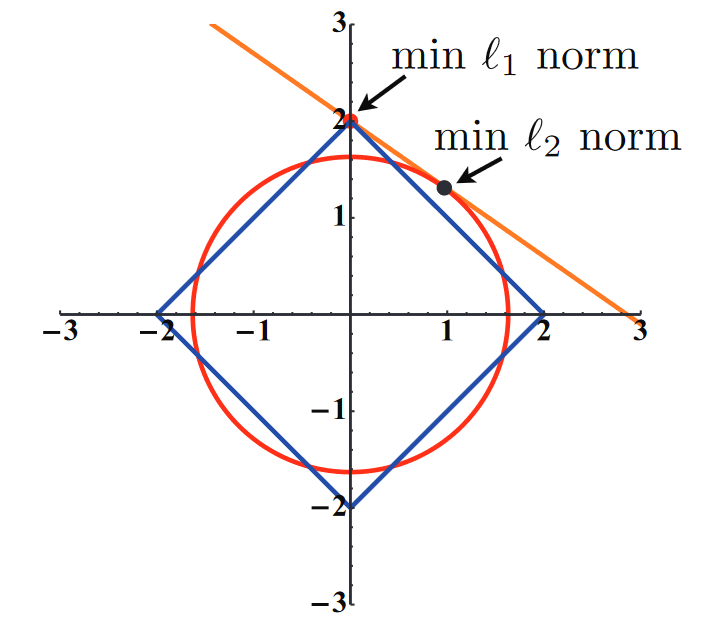
\includegraphics[scale=0.5]{lnorm}
    \caption{Illustration of constant $\ell_1$ norm surfaces in $R^2$. The circle is a constant $\ell_2$ norm surface and the diamond is a constant $\ell_1$ norm surface. The straight line indicates the possible solutions to the under determined problem $10y + 7x = 20$. A sparse solution to this problem is the solution where one of the variables is zero and the other is not; in other words it is at the intersection of the straight line and the axes. Minimizing the $\ell_2$ norm of this system will result in a dense solution, whereas minimizing the $\ell_1$ norm will yield a sparse solution\cite{PhysRevB.88.155105}. (Note: When using someones figure am I supposed to use their caption or make my own? The above is the original caption.)}
    \label{fig:l1norm}
\end{figure}

\section{Methods and Setup}
This work examined 998 structures as an initial training set for the cluster expansion. An additional 115 structures were added to the set in order to further refine the CE around the convex hull. A sample input file for Quantum Espresso is provided in Appendix but some key values used are as follows: convergence threshold of 3e-6, mixing beta of 0.2 and an plane wave energy cutoff of 40.0. Furthermore, a relatively dense K-point mesh was used that had a total number of K-points equal to
$$ \text{K-points}_{total} = \frac{8000}{N_{atoms}} $$
scaled in each lattice vector proportional to its magnitude. The more atoms relax off lattice site the less accurate, and viable the cluster expansion becomes so ensuring the structure relaxes is important.\cite{2017arXiv170103080N}. In order to properly capture the atomic relaxation for the structures we ran the calculations twice. The final positions of the atoms in the first run were used as the input positions for the second DFT calculations. We then calculated the formation enthalpy of each structure using

$$ \text{formation enthalpy} = \frac{E_{\text{total alloy}}}{N_{\text{alloy}}} - (x_A \frac{E_A}{N
_A} + x_B \frac{E_B}{N
_B} + x_C \frac{E_C}{N
_C}) $$

where x is the concentrations of species A, B, and C, and their respective energy of a pure configuration E. N is the number of each atom time in a pure unit cell. The formation enthalpy of the sample structures were then compiled into necessary inputs for use in UNCLE.

UNCLE was used to handle the cluster expansion for the system and the groundstate search. Default values were used with the exception of the CS input files. Here we used J cuttoff of 0.001 and sigma correlation value of 1.0.

\section{Results}

Pending further refinement of data to ensure claims described in abstract are met.

discussion of error of CE fit (normalized R^2 values)
histogram of R^2 values

figure of convex hull

table of ground state structure energies (better placed in appendix?)

\section{conclusion}
The location of the ground states found in the concentration domain through a combination of first principle calculations and cluster expansion indicates that there are structures in the cobalt rich concentration region that could be viable candidate alloys. The thermodynamic monte carlo suggests that the selected ground states have high transition temperatures and could therefore have application as super alloys.

\bibliographystyle{unsrt}
\bibliography{citations}

\end{document}
